

\subsection{Ciprofloxacin derivative}

%Ciprofloxacin \compound{cmpd:cip} (see \ref{fgr:cip_num}) is second-generation fluoroquinolone antibiotic used to treat both Gram-positive and Gram-negative bacterial infections\cite{Oliphant2002}.
%The structure-activity relationships for ciprofloxacin have been investigated \cite{Renau1996} and positions 2 and 7 were found not to cause loss of activity. It was therefore decided that alkyne tails would be added at these positions giving two derivatives of ciprofloxacin, \compound{cmpd:Y4Cip} and \compound{cmpd:pipciphex} (see \ref{sch:cip_anas}).

\todo{put intro in intro}

%Three derivatives of ciprofloxacin modified at the free piperazine N were synthesised. These contained a six-carbon alkyl chain with a terminal alkyne, a six-carbon acyl chain with a terminal alkyne and a three carbon acyl chain with a terminal alkyne.

\subsubsection{Retrosynthesis of ciprofloxacin derivative \compound{cmpd:Y4Cip}}

The retrosynthesis of ciprofloxacin derivative \compound{cmpd:Y4Cip} is shown in \ref{sch:Y4Cip_retro}. The disconnection to an alkynyl piperazine \compound{cmpd:Y4Cip} and a commercially available ciprofloxacin precursor \compound{cmpd:Clcip} was chosen based on a study by Renau \textit{et al.}, who found this route to be "...superior to previous reports which involved alkylation of piperazine with an appropriate alkyl halide." \cite{Renau1996,JPS:JPS2600571210}. 

It was envisaged that the alkynyl piperazine \compound{cmpd:Y4Cip} could be prepared from mono-Boc-protected piperazine \compound{cmpd:pipboc} and hex-5-ynal \compound{cmpd:hexynal} using conditions similar to those used by Renau \textit{et al.}\cite{Renau1996}.

Unlike the aldehydes and ketones used by Renau \textit{et al.}\cite{Renau1996}, hex-5-ynal \compound{cmpd:hexynal} is not commercially available and so it was hoped that this could be prepared by oxidation of hex-5-ynol \compound{cmpd:hexynol}.

%This can be achieved by reductive amination of hex-5-ynal \compound{cmpd:hexynal} with 1-boc-piperazine \compound{cmpd:pipboc} followed by deprotection to form the alkyl piperazine \compound{cmpd:hexpip}. 
%S$_N$Ar coupling of the piperazine derivative with ciprofloxacin precursor \compound{cmpd:Clcip} leads to the final derivative \compound{cmpd:Y4Cip}.

\begin{scheme}[H]
	\begin{center}
		\schemeref[hexynol]{cmpd:hexynol}
		\schemeref[hexynal]{cmpd:hexynal}
		\schemeref[pipboc]{cmpd:pipboc}
		\schemeref[hexpipboc]{cmpd:hexpipboc}
		\schemeref[hexpip]{cmpd:hexpip}
		\schemeref[Clcip]{cmpd:Clcip}
		\schemeref[hexpipcip]{cmpd:Y4Cip}
		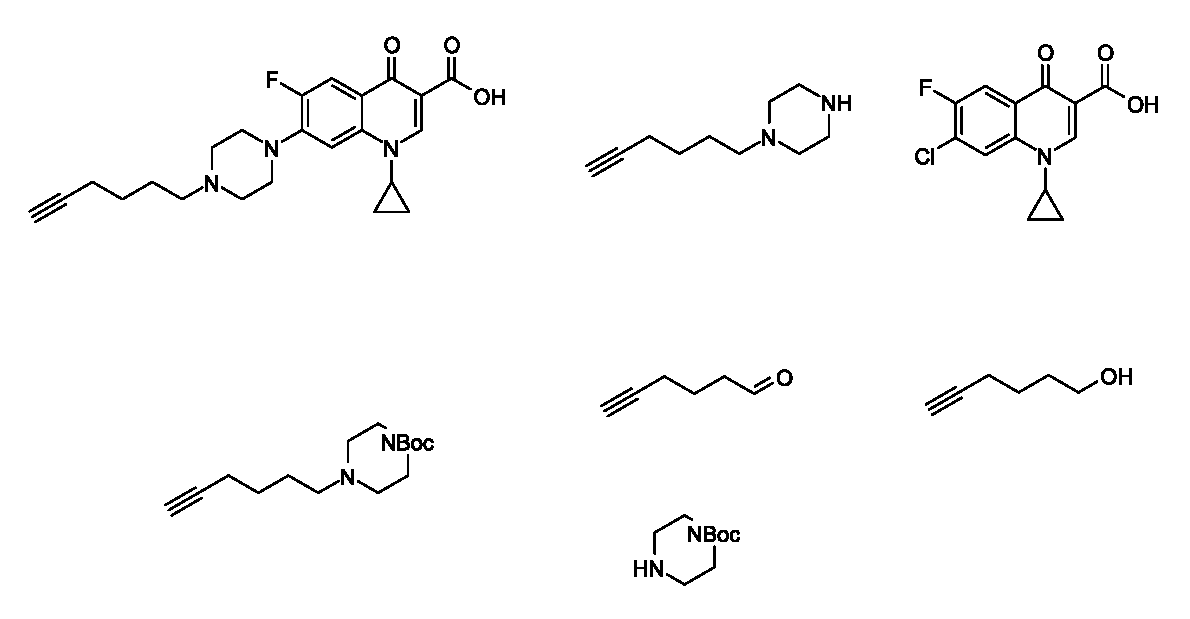
\includegraphics[scale=1]{hexpipcip_retro}
		\caption{The retrosynthesis of \compound{cmpd:Y4Cip}. \label{sch:Y4Cip_retro}}
	\end{center}
\end{scheme}

\subsubsection{Synthesis of ciprofloxacin derivative \compound{cmpd:Y4Cip}}

The synthesis of ciprofloxacin derivative \compound{cmpd:Y4Cip} is shown in \ref{sch:Y4Cip_synth}. Hex-5-ynal \compound{cmpd:hexynal} was prepared by PCC oxidation of hex-5-ynol \compound{cmpd:hexynol} in good yield according to the procedure described by Kocsis \textit{et al.} \cite{Kocsis2012}. 

Renau \textit{et al.}\cite{Renau1996} used sodium cyanoborohydride to facilitate the reductive amination of hex-5-ynal \compound{cmpd:hexynal} and 1-Boc-piperazine \compound{cmpd:pipboc}. However, it was decided to attempt this transformation using the less toxic sodium triacetoxyborohydride following a procedure reported by Abdel-Magid \textit{et al.} \cite{Abdel-Magid1996}. This reaction yielded compound \compound{cmpd:hexpipboc} in excellent yield, which was deprotected using TFA using the procedure described by Renau \textit{et al.}\cite{Renau1996} to give the alkynyl piperazine \compound{cmpd:hexpip} quantitatively. 

The alkynyl piperazine \compound{cmpd:hexpip} was refluxed in MeCN with the ciprofloxacin precursor \compound{cmpd:Clcip} according to the procedure described by Renau \textit{et al.}\cite{Renau1996}, however the reaction did not proceed. Addition of 2 eq. of \ce{NEt3} did not lead to reaction, however it was found that refluxing in neat \ce{NEt3} led to conversion to the final ciprofloxacin derivative \compound{cmpd:Y4Cip}.

With a small sample of the final product in hand, less harsh conditions were sought for a larger-scale version of the final reaction. Mircowave irradiation at 115 $^{\circ}$C was used, following a procedure by Reddy \textit{et al.}\cite{Reddy2001}. DMSO and NMP were tested as solvents, with or without the addition of TEA. The reactions were monitored using LCMS, and NMP without TEA was found to give the highest conversion. 

Work-up of this reaction proved difficult, with an unknown dark brown viscous liquid being formed which was difficult to separate from the white solid product. A pure sample was obtained by recrystalisation from EtOAc, but the yield was rather poor (11.8 \%). The reaction was observed to stall after a certain point, while still having some of the ciprofloxacin precursor \compound{cmpd:Clcip} present. The alkynyl piperazine \compound{cmpd:hexpip} was not observed by TLC despite having been added in two-fold excess, suggesting that it degraded to a by-product before having chance to react. 

Further attempts to refine this reaction might involve lower temperatures, higher ratios of the alkynyl piperazine \compound{cmpd:hexpip} or improvement of the purification, e.g. by finding better precipitation conditions or by using reverse-phase chromatography. A Buchwald-Hartwig coupling or Ullmann reaction could also be attempted, but, as seen later, coordination of ciprofloxacin to Cu can hinder catalysis.

\begin{scheme}[H]
	\begin{center}
		\schemeref[hexynol]{cmpd:hexynol}
		\schemeref[hexynal]{cmpd:hexynal}
		\schemeref[pipboc]{cmpd:pipboc}
		\schemeref[hexpipboc]{cmpd:hexpipboc}
		\schemeref[hexpip]{cmpd:hexpip}
		\schemeref[Clcip]{cmpd:Clcip}
		\schemeref[hexpipcip]{cmpd:Y4Cip}
		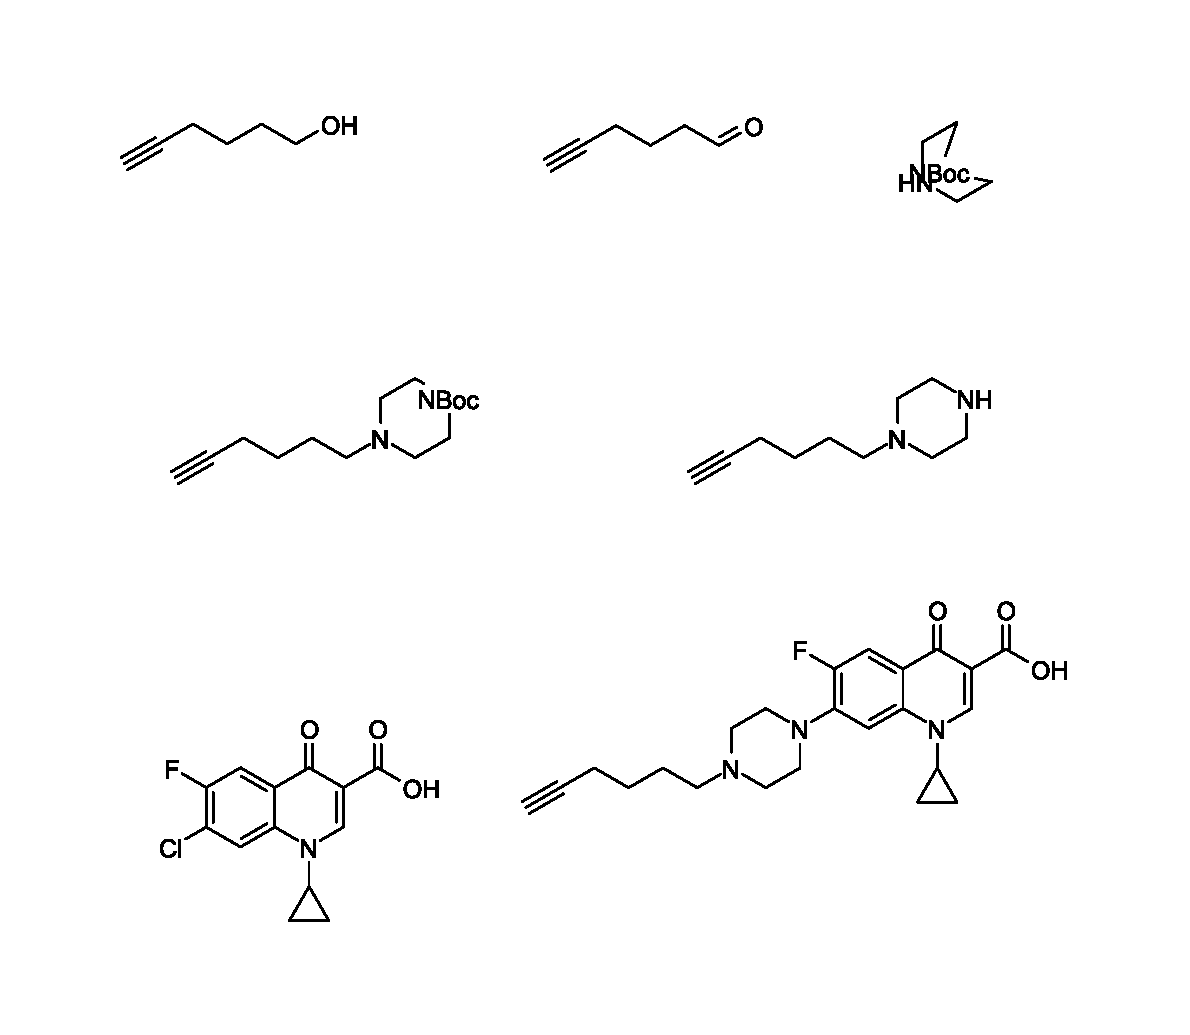
\includegraphics[scale=1]{hexpipcip_synth}
		\caption{The synthesis of \compound{cmpd:Y4Cip}. 
		a) Pyridinium chlorochromate, \ce{CH2Cl2}, r.t., 5 h, 72 \%.
		b) \ce{NaBH(AcO)3}, 1,2-dichloroethane, r.t., 10.5 h, 99 \%.
		c) TFA, r.t., 1 h, 100 \%.
		d) NMP, microwave, 115 $^{\circ}$C 24 h, 11.8 \%.
		\label{sch:Y4Cip_synth}}
	\end{center}
\end{scheme}

\subsection{Trimethoprim derivative}

The synthesis of trimethoprim derivative \compound{cmpd:Y4Tri} is shown in \ref{sch:Y4Tri_synth}. Trimethoprim was selectively deprotected using HBr (aq.) using a procedure described by Jing \textit{et al.}\cite{Jing2013} to form \compound{cmpd:HOTri}. A slightly longer reaction time (40 min vs 20 min) probably led to the yield being slightly somewhat lower than that obtained by Jing \textit{et al.}. 
The main impurity was asymmetrically di-demethylated trimethoprim, which could be identified by the presence of two aryl peaks at 6.41 (d, J=2.0 Hz, 1 H) and 6.34 (d, J=2.0 Hz, 1 H) and a corresponding methyl peak at 3.82 (s, 3 H) in the crude NMR.

The alkynyl trimethoprim derivative \compound{cmpd:Y4Tri} was synthesised from the demethylated trimethoprim \compound{cmpd:HOTri} and 6-chloro-1-hexyne \compound{cmpd:Y4Cl} using a \ce{Cs2CO3}-catalysed S$_N$2 reaction similar to that used by Jing \textit{et al.}.
\todo{weigh Y4Tri then discuss}

\begin{scheme}[H]
	\begin{center}
		\schemeref[Tri]{cmpd:Tri}
		\schemeref[TriOH]{cmpd:HOTri}
		\schemeref[Cl4Y]{cmpd:Y4Cl}
		\schemeref[Y4Tri]{cmpd:Y4Tri}
		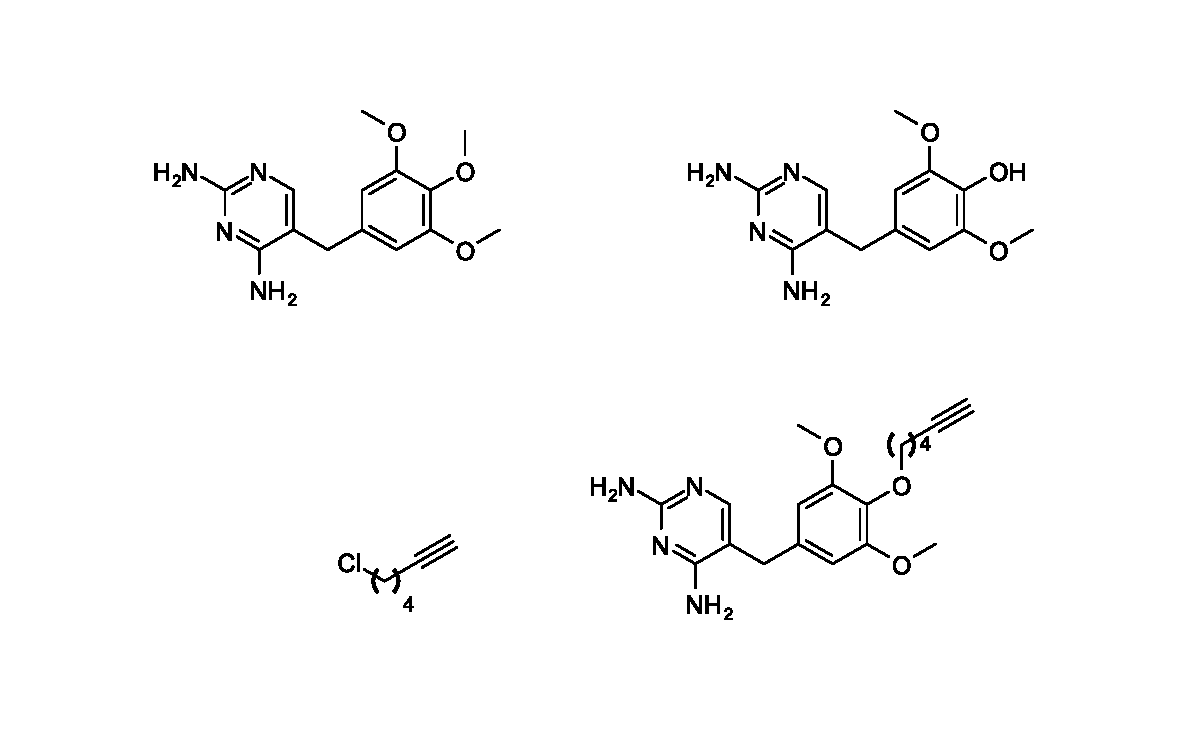
\includegraphics[scale=1]{Y4Tri_synth}
		\caption{The synthesis of \compound{cmpd:Y4Tri}.
		a) HBr (aq.), 100 $^{\circ}$C, 40 min, 43.4 \%. 
		b) \ce{Cs2CO3}, DMF, 70 $^{\circ}$C, 7 h, 19.6 \%.
		\label{sch:Y4Tri_synth}}
	\end{center}
\end{scheme}

